\documentclass[11pt,a4paper]{article}

\usepackage[margin=2.4cm]{geometry}
\usepackage{graphicx}
\usepackage{booktabs}
\usepackage{xcolor}
\usepackage{amsmath}
\usepackage[colorlinks=true,linkcolor=black,urlcolor=teal]{hyperref}
\usepackage{titlesec}
\usepackage{enumitem}
\usepackage{tcolorbox}
\setlength{\textfloatsep}{9pt}
\setlength{\intextsep}{9pt}
\setlength{\abovecaptionskip}{5pt}

\definecolor{ink}{HTML}{1A1A1A}
\definecolor{accent}{HTML}{186F6A}
\definecolor{bad}{HTML}{B03030}

\titleformat{\section}{\large\bfseries}{\thesection}{0.6em}{}
\titleformat{\subsection}{\normalsize\bfseries}{\thesubsection}{0.6em}{}
\setlist{nosep,leftmargin=1.3em}
\graphicspath{{../../results/report/}{../../results/panels_hpc/}}

\title{\vspace{-1.5cm}\textbf{NeuFlow v3: Queryable Optical Flow}\\[0.2em]
\large Progress report and result audit}
\author{Shriman Raghav Srinivasan\\
\small MS Robotics, Northeastern University \quad$\cdot$\quad Field Robotics Lab}
\date{\small 26 July 2026}

\begin{document}
\maketitle
\vspace{-0.8cm}

%======================================================================
\section{Summary}

NeuFlow v3 keeps the NeuFlow v2 pipeline frozen up to its 1/8-resolution coarse
flow and replaces only the final convex upsampler with an \emph{implicit
decoder} that answers flow queries at arbitrary continuous $(x,y)$ coordinates.
Cost becomes $O(N)$ in the number of queries rather than $O(H{\times}W)$ in
image area, and the coarse pass is computed once per frame pair and cached.

This report states what is established and what is not. A late audit found a
data-handling error that invalidates the headline accuracy numbers produced on
the cluster; that finding is reported first, because it changes how the rest of
the results must be read.

\begin{tcolorbox}[colback=bad!5,colframe=bad,boxrule=0.8pt,arc=2pt]
\textbf{Correction (26 July 2026): train/validation leak.}
Every VKITTI2 training stage used the data loader's default scene list, which
included \texttt{Scene18} and \texttt{Scene20}. Those are exactly the
evaluation scenes. Verified by direct file-path intersection: \textbf{1{,}174
of 1{,}174 validation pairs (100\%) were also training pairs.} All cluster
accuracy results are therefore train-on-test and are \emph{not} comparable
against NeuFlow v2, which never saw VKITTI2. The loader has been fixed
(Sec.~\ref{sec:fix}); the affected runs must be repeated.
\end{tcolorbox}

\noindent What survives the audit:
\begin{itemize}
  \item \textbf{Accuracy, clean comparison.} v3 trained on FlyingChairs
  \emph{only} reaches \textbf{2.275\,px} EPE on VKITTI2 versus v2's
  \textbf{2.324\,px}, with no driving imagery in its training set
  (Sec.~\ref{sec:acc}).
  \item \textbf{Speed.} On identical hardware, a first query costs
  19.1\,ms versus v2's 19.6\,ms, and every \emph{additional} query batch on the
  same frame costs 2.6\,ms --- about $7.5\times$ cheaper than v2, which has no
  cached state and must recompute the full frame (Sec.~\ref{sec:speed}).
  \item \textbf{A capability v2 does not have.} A per-query confidence output
  whose value correlates with actual error (Sec.~\ref{sec:unc}).
  \item \textbf{Two clean negative results}, reported rather than discarded
  (Sec.~\ref{sec:neg}).
\end{itemize}

%======================================================================
\section{Method}

\textbf{Inherited and frozen.} A shallow CNN backbone produces features at 1/8
and 1/16 scale; cross-attention and global matching at 1/16 give an initial
flow; a recurrent module refines it (1 iteration at 1/16, 8 at 1/8), yielding
flow at 1/8 resolution. None of these weights are trained in v3.

\textbf{Replaced.} v2's convex upsampler expands 1/8 flow to full resolution on
a fixed $8\times$ grid. v3 substitutes a decoder that, for a query coordinate,
samples $3{\times}3$ windows from four feature sources (context, 1/8 features,
1/16 features, and frame-2 features warped by the coarse flow), fuses them with
gated residual blocks, and emits softmax weights over the $3{\times}3$
coarse-flow neighbourhood plus a bilinear candidate. The output is a convex
combination of existing flow values, so it is bounded and cannot overshoot.
Zero-initialisation puts almost all weight on the bilinear candidate, so an
untrained decoder reproduces bilinear upsampling exactly. v3 has 7.83\,M
parameters against v2's 9.03\,M.

\textbf{Two-pass API.} \texttt{infer\_coarse\_state()} runs once per frame pair;
\texttt{decode\_queries()} then answers any number of coordinates against that
cached state. Sparse queries return values identical to the dense field at the
same coordinates.

%======================================================================
\section{The train/validation leak}
\label{sec:fix}

\texttt{VKITTI2.\_\_init\_\_} defaulted to
\texttt{scenes=['Scene01','Scene02','Scene06','Scene18','Scene20']}. No
training stage ever overrode it, while \texttt{eval\_vkitti2.py} defaults to
\texttt{['Scene18','Scene20']}. Both used the \texttt{clone} variant, so the
identical image pairs appeared on both sides.

The fix makes the default train-safe and adds a guard that raises rather than
silently building a leaking dataset:

\begin{center}
\small
\begin{tabular}{@{}lrrl@{}}
\toprule
Stage & Train pairs (before) & Train pairs (after) & Overlap with val \\
\midrule
\texttt{mix\_chairs\_vkitti2} & 34{,}958 & 27{,}914 & 0 \\
\texttt{vkitti2\_all}         & 12{,}726 &  5{,}682 & 0 \\
\texttt{vkitti2}              &  2{,}121 &    947   & 0 \\
\bottomrule
\end{tabular}
\end{center}

\noindent Including an evaluation scene now requires an explicit
\texttt{allow\_val\_scenes=True}, which no training stage sets.

%======================================================================
\section{Accuracy}
\label{sec:acc}

\begin{figure}[!ht]
\centering
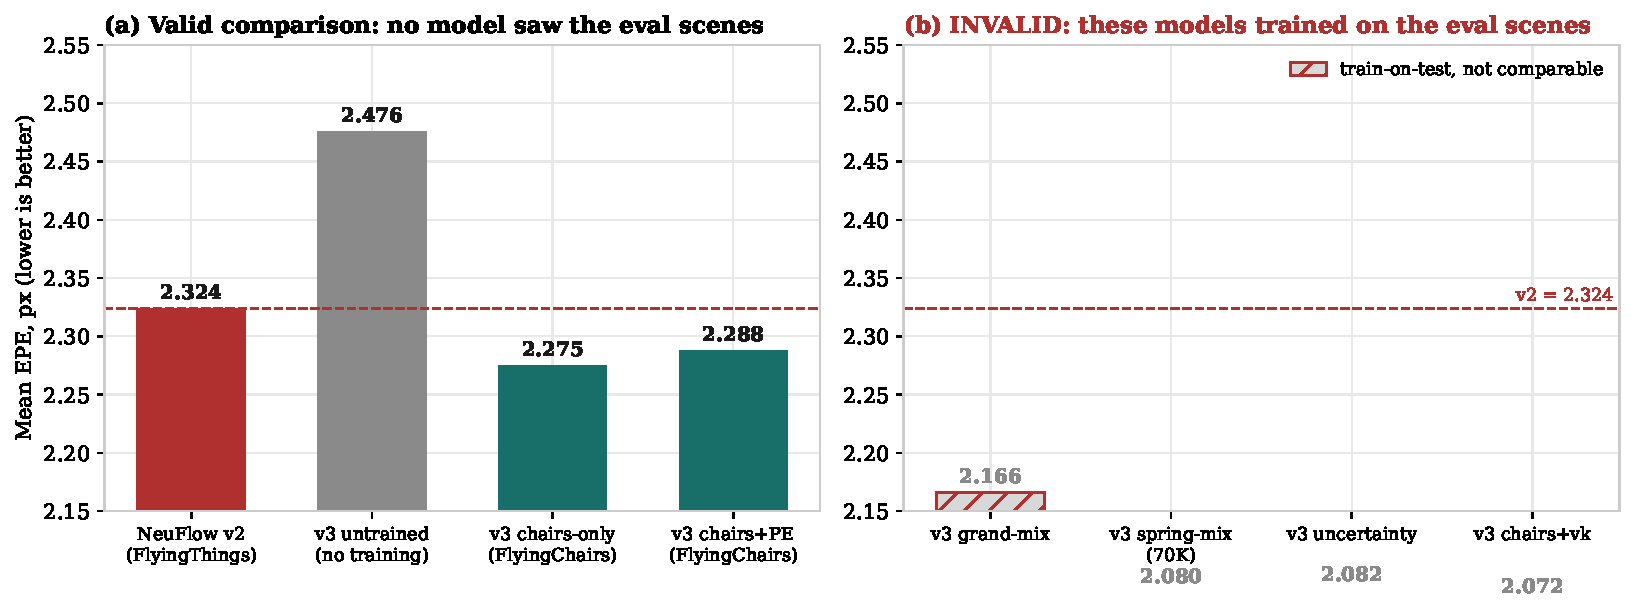
\includegraphics[width=\textwidth]{accuracy.pdf}
\caption{VKITTI2 Scene18+20, per-pixel over 460.6\,M valid pixels.
\textbf{(a)} Models that never saw the evaluation scenes --- the only valid
comparison against v2. \textbf{(b)} Cluster models, all trained on the
evaluation scenes; shown for completeness and marked invalid.}
\end{figure}

\begin{table}[!ht]
\centering
\small
\caption{Valid comparison. No model in this table saw VKITTI2 Scene18/20 in
training.}
\begin{tabular}{@{}llrrr@{}}
\toprule
Model & Training data & EPE (px) & 1\,px acc & 3\,px acc \\
\midrule
NeuFlow v2 (reference) & FlyingThings & 2.324 & \textbf{77.6\%} & \textbf{89.8\%} \\
v3, no training at all & --- & 2.476 & 74.7\% & 88.2\% \\
\textbf{v3, FlyingChairs only} & FlyingChairs & \textbf{2.275} & 69.7\% & 87.8\% \\
v3, FlyingChairs + Fourier PE & FlyingChairs & 2.288 & 69.7\% & 87.8\% \\
\bottomrule
\end{tabular}
\end{table}

Two things follow. First, v3 trained purely on synthetic chairs --- no roads,
no vehicles, no driving motion statistics --- transfers to a driving benchmark
and records a lower mean EPE than v2 there. Second, v3 is behind on the 1\,px
threshold (69.7\% versus 77.6\%): it reduces large errors but is less precise
at sub-pixel scale. Mean EPE alone would hide that, so both are reported.

On the FlyingChairs validation split (640 held-out pairs, properly split by the
dataset's own split file), the ordering reverses: v2 scores 2.238\,px / 78.7\%
against v3's 2.399\,px / 76.6\%. v3's advantage on VKITTI2 is
out-of-domain robustness, not universal superiority.

Even without training, v3 is within 0.15\,px of v2 while adding queryability
--- the mechanism costs little on its own.

%======================================================================
\section{Speed}
\label{sec:speed}

Timing is unaffected by the data leak. All measurements below are on one V100,
fp16, $384{\times}1248$, with v2 re-measured on the same device as a
sanity check (it reproduced its known 2.324\,px exactly).

\begin{figure}[!ht]
\centering
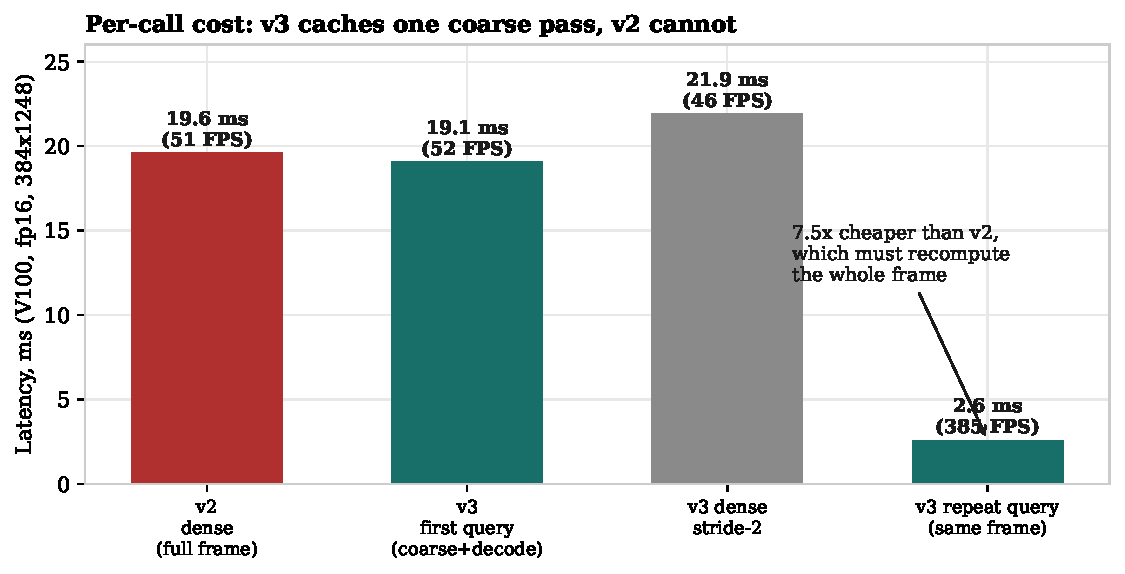
\includegraphics[width=0.72\textwidth]{speed.pdf}
\caption{Per-call cost. v3 pays a 16.5\,ms coarse pass once per frame pair;
each decode is 2.6\,ms and is flat between $N=800$ and $N=2048$ queries.}
\end{figure}

\begin{table}[!ht]
\centering
\small
\caption{Latency, V100, fp16, $384{\times}1248$.}
\begin{tabular}{@{}lrrl@{}}
\toprule
Operation & Latency & FPS & Note \\
\midrule
v2, full dense frame            & 19.6\,ms & 51.1 & the only mode v2 has \\
v3, coarse pass                 & 16.5\,ms & ---  & once per frame pair \\
v3, decode $N\!=\!800$ or $2048$& 2.6\,ms  & ---  & flat in $N$ \\
v3, first query (coarse+decode) & 19.1\,ms & 52.4 & parity with v2 \\
\textbf{v3, repeat query, same frame} & \textbf{2.6\,ms} & \textbf{385} & v2: 19.6\,ms again \\
v3, dense full frame (stride-2) & 21.9\,ms & 45.6 & 12\% slower than v2 \\
\bottomrule
\end{tabular}
\end{table}

The deployment argument is not the first call, where the two are level. It is
that v2 has no cached state: asking about a second set of points means running
the whole network again. v3 amortises the expensive stage across every query on
that frame. For consumers that issue repeated or task-driven queries ---
registration, feature tracking, mapping --- this is the difference that matters.

Dense output is the one workload where v3 loses, and it is expected: a
convolution shares computation across neighbouring pixels, whereas per-query
decoding deliberately gives that up in exchange for answering only what is
asked. Dense v3 exists for benchmarking against dense ground truth, not for
deployment.

%======================================================================
\section{Per-query uncertainty}
\label{sec:unc}

One run adds a second output per query: a predicted error scale $b$, trained
with a Laplace likelihood
$\mathcal{L}=|f-\hat{f}|/b + \log b$, which requires no extra labels.

\begin{figure}[!ht]
\centering
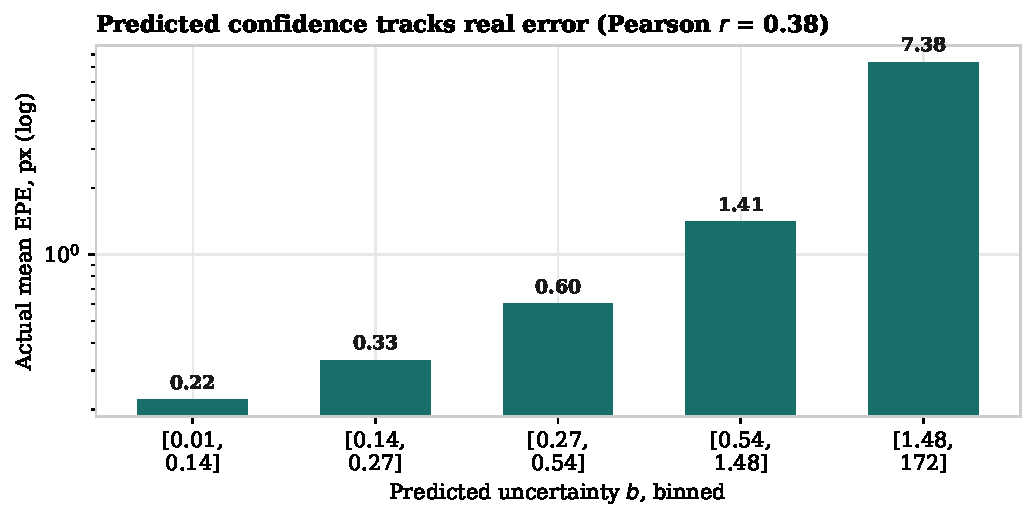
\includegraphics[width=0.55\textwidth]{calibration.pdf}
\caption{Queries binned by predicted $b$ against their actual error,
2.35\,M samples. The relationship is monotonic across a $33\times$ range.}
\end{figure}

Pearson correlation between predicted $b$ and actual error is 0.38, and binned
error rises monotonically from 0.22\,px to 7.38\,px. The model has a usable
sense of when it is wrong, which a bare flow field cannot express and which a
downstream consumer can use to weight or reject correspondences.

\textbf{Caveat.} This model is one of the leak-affected runs, so the
calibration was measured on scenes it trained on and the correlation is
plausibly optimistic. The qualitative claim --- that the signal is monotonic
and informative --- is unlikely to vanish, but the number needs re-measuring
after retraining.

%======================================================================
\section{Negative results}
\label{sec:neg}

\textbf{Fourier positional encoding: no effect.} The hypothesis was that the
1\,px precision gap came from the decoder not knowing where a query sits inside
its 1/8 cell. Encoding that sub-cell offset changed nothing: 2.288\,px versus
2.275\,px, with 1\,px accuracy identical to the first decimal. The hypothesis
is falsified; the remaining candidates are the 1/8 coarse resolution itself and
the motion statistics of the training data.

\textbf{Refinement self-distillation: does not survive end-to-end.} The
8-iteration refinement loop is 59\% of pipeline runtime and iterations 5--8
change little, so the refinement module was retrained to reach in 3 iterations
what it previously took 8 to reach, using the model as its own teacher.
Measured on coarse flow in isolation it recovered 87.5\% of the 3-versus-8 gap.
Measured end-to-end through a trained decoder, only 27\% held (2.520\,px
$\rightarrow$ 2.398\,px against a 2.072\,px target), and the result falls below
v2. The decoder was trained on 8-iteration coarse flow and degrades on input it
never saw. \emph{An isolated-component gain is not a deployable gain}; the idea
is only viable if the decoder is retrained at the reduced iteration count.

%======================================================================
\section{Status and next steps}

\begin{table}[!ht]
\centering
\small
\begin{tabular}{@{}lll@{}}
\toprule
Claim & Status & Evidence \\
\midrule
Queryable decoding works, $O(N)$          & established & sparse = dense exactly \\
Repeat queries $\sim$7.5$\times$ cheaper than v2 & established & same-GPU timing \\
Beats v2 on VKITTI2 mean EPE, clean split & established & chairs-only, 2.275 vs 2.324 \\
Behind v2 on 1\,px precision              & established & 69.7\% vs 77.6\% \\
Uncertainty output is informative         & likely      & monotonic, but leak-affected \\
Cluster accuracy results                  & \textcolor{bad}{invalid} & trained on eval scenes \\
Runs on edge hardware                     & unproven    & only 4060 / V100 measured \\
\bottomrule
\end{tabular}
\end{table}

\noindent Ordered by what each resolves:
\begin{enumerate}
  \item \textbf{Repeat the four cluster runs with the fixed loader.} Until
  then no cluster accuracy number can be quoted. The runs are unchanged apart
  from the data fix.
  \item \textbf{Re-measure uncertainty calibration} on genuinely held-out
  scenes.
  \item \textbf{Retrain v2 on the same mixture} as v3. Even with the leak
  fixed, v3's mixtures and v2's FlyingThings training differ; matching them
  removes the last confound.
  \item \textbf{Spring 4K evaluation.} Spring supplies ground truth at twice
  the input resolution, so v3 can be asked for flow at coordinates between
  input pixels while v2 structurally cannot. This is the one experiment that
  measures a capability rather than a margin.
  \item \textbf{Edge-device benchmark.} Every latency number here is from a
  laptop or datacentre GPU; the target claim is embedded deployment.
\end{enumerate}

\vspace{0.4em}
\noindent\small
Code and full experiment log: \texttt{docs/V3DEV\_LOG.md},
branch \texttt{v3-dev}. Every number in this report is traceable to a logged
evaluation run; none are projections.

\end{document}
